\documentclass[10pt]{beamer}

\usetheme{Oxygen}
\usepackage{hyperref}
\usepackage[compatibility=false]{caption}
\usepackage{thumbpdf}
\usepackage{wasysym}
\usepackage{ucs}
\usepackage[utf8]{inputenc}
\usepackage{pgf,pgfarrows,pgfnodes,pgfautomata,pgfheaps,pgfshade}
\usepackage{verbatim}
\usepackage{listing}
\usepackage{url}
\usepackage{cite}
\usepackage{minted}

\pdfinfo
{
  /Title       (iOS Application Development)
  /Creator     (TeX)
  /Author      (Chris Zelenak)
}


\title{iOS Application Development}
\subtitle{Day 2}
\author{Chris Zelenak}
\date{10/05/2010}

\begin{document}



\frame{\titlepage}

\section*{}
\begin{frame}
  \frametitle{Outline}
  \tableofcontents[section=1,hidesubsections]
\end{frame}

\AtBeginSection[]
{
  \frame<handout:0>
  {
    \frametitle{Outline}
    \tableofcontents[currentsection,hideallsubsections]
  }
}

\AtBeginSubsection[]
{
  \frame<handout:0>
  {
    \frametitle{Outline}
    \tableofcontents[sectionstyle=show/hide,subsectionstyle=show/shaded/hide]
  }
}

\newcommand<>{\highlighton}[1]{%
  \alt#2{\structure{#1}}{{#1}}
}

\newcommand{\icon}[1]{\pgfimage[height=1em]{#1}}

 

  
    
% BEGIN SECTION Images
\section{Images}
\begin{frame}[fragile]
  \frametitle{Images}
  1. Images
\end{frame}


    
\begin{frame}[fragile]
  \frametitle{The UIImage}
  A way to represent a bytestream

\end{frame}

\begin{frame}[fragile]
  \frametitle{The UIImage}
  Does NOT give you access to the underlying image data

\end{frame}

\begin{frame}[fragile]
  \frametitle{The UIImage}
  Can be made from any given iPhone UI screen

\end{frame}

\begin{frame}[fragile]
  \frametitle{The UIImage}
  Carries with it a lower level CGImageRef object \begin{minted}[resetmargins=true,fontsize=\footnotesize]{objectivec}

  CGImageRef theImage = [aUIImage CGImage];

  \end{minted}

\end{frame}

\begin{frame}[fragile]
  \frametitle{The UIImage}
  Can be loaded in cache form with \begin{minted}[resetmargins=true,fontsize=\footnotesize]{objectivec}

  UIImage * img = [UIImage imageNamed:@"ImageFilename.png"];

  \end{minted}
or loaded in no-cache form with \begin{minted}[resetmargins=true,fontsize=\footnotesize]{objectivec}

  NSBundle * bnd = [NSBundle mainBundle];
  NSString * path = [bnd pathForResource:@"ImageFilename" ofType:@"png"];
  UIImage * img = [[UIImage alloc] initWithContentsOfFile:path];

  \end{minted}

\end{frame}

\begin{frame}[fragile]
  \frametitle{The UIImage}
  UIImage can handle most basic image types: PNG, JEPG, GIF, ICO, BMP, TIF..

\end{frame}

\begin{frame}[fragile]
  \frametitle{The UIImage}
  But the fastest way to load and draw images will typically be with PNGs.

\end{frame}

    
\begin{frame}[fragile]
  \frametitle{UIImageView and UIButton}
  UIImageView provides a simple way to put an image on the screen, w/ no interaction

\end{frame}

\begin{frame}[fragile]
  \frametitle{UIImageView and UIButton}
  \begin{listing}[H]
    \begin{minted}[resetmargins=true,fontsize=\footnotesize]{objectivec}

  UIImageView * v = [[UIImageView alloc]
                      initWithFrame:CGRectMake(0.0, 0.0, 200.0, 200.0)];
  UIImage * someImage = [UIImage imageNamed:@"screenImage.png"];
  [v setImage:someImage];
  [someView addSubview:v];
  [v release];

  \end{minted}
    \caption{Loading a UIImageView with an image}
    \label{listing:27}
  \end{listing}

\end{frame}

\begin{frame}[fragile]
  \frametitle{UIImageView and UIButton}
  UIButton can also show an image instead of a rounded rectangle.  It can display different images for both foreground and background based on its current state as well.

\end{frame}

\begin{frame}[fragile]
  \frametitle{UIImageView and UIButton}
  \begin{listing}[H]
    \begin{minted}[resetmargins=true,fontsize=\footnotesize]{objectivec}

  UIButton * b = [UIButton buttonWithType:UIButtonTypeCustom];
  [b setImage:[UIImage imageNamed:@"btnImage.png"]
     forState:UIControlStateNormal];
  [b setBackgroundImage:[UIImage imageNamed:@"btnImageSelectedBG.png"]
               forState:UIControlStateSelected];
  [someView addSubview:b];

  \end{minted}
    \caption{Loading a UIButton with an image}
    \label{listing:28}
  \end{listing}

\end{frame}

    
\begin{frame}[fragile]
  \frametitle{Lab 4}
  Create a detail UITableViewController

\end{frame}

\begin{frame}[fragile]
  \frametitle{Lab 4}
  Load in class images in header with student name

\end{frame}

\begin{frame}[fragile]
  \frametitle{Lab 4}
  Push UITableViewController onto UINavigationController stack

\end{frame}

    

% END SECTION Images
   
  

  
    
% BEGIN SECTION More about UIView and Core Graphics
\section{More about UIView and Core Graphics}
\begin{frame}[fragile]
  \frametitle{More about UIView and Core Graphics}
  2. More about UIView and Core Graphics
\end{frame}


    
\begin{frame}[fragile]
  \frametitle{What comes with UIView}
  Any UIView can have its background color, overall opacity,  dimensions and overall coordinate transform (CGAffineTransform)

\end{frame}

\begin{frame}[fragile]
  \frametitle{What comes with UIView}
  Any UIView can contain any number of subviews

\end{frame}

\begin{frame}[fragile]
  \frametitle{What comes with UIView}
  Any UIView can have specific autoresizing behavior applied to it when its parent view changes

\end{frame}

\begin{frame}[fragile]
  \frametitle{What comes with UIView}
  Any UIView can automatically resize its subviews when its dimensions change

\end{frame}

\begin{frame}[fragile]
  \frametitle{What comes with UIView}
  Any UIView subclass can choose to respond to direct touch events

\end{frame}

\begin{frame}[fragile]
  \frametitle{What comes with UIView}
  Any UIView can optionally choose to blit its contents directly to the screen with Core Graphics

\end{frame}

    
\begin{frame}[fragile]
  \frametitle{Views and subviews}
  The subviews a UIView has are contained within the subviews property of a view

\end{frame}

\begin{frame}[fragile]
  \frametitle{Views and subviews}
  You can see the subviews of a view layed out in Interface Builder by expanding the View in the Document view \begin{figure}[htb]
  \begin{center}

  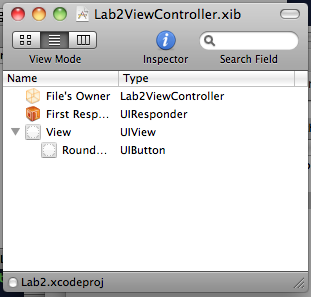
\includegraphics[scale=0.5]{UIViewExpand.png}

  \caption{Expanding the contents of a UIView}
  \end{center}
  \end{figure}

\end{frame}

\begin{frame}[fragile]
  \frametitle{Views and subviews}
  Views overlay each other based on the order they are added to the parent view; you can swap their order by using UIView methods like \begin{minted}[resetmargins=true,fontsize=\footnotesize]{objectivec}

  -(void) bringSubviewToFront:(UIView *)view;
  -(void) sendSubviewToBack:(UIView *)view;
  -(void) exchangeSubviewAtIndex:(NSInteger)idx withSubviewAtIndex:(NSInteger)idx;

  \end{minted}

\end{frame}

    
\begin{frame}[fragile]
  \frametitle{Events and control events}
  Any UIView subclass can override the methods
\begin{listing}[H]
    \begin{minted}[resetmargins=true,fontsize=\footnotesize]{objectivec}

  - (void)touchesBegan:(NSSet *)touches withEvent:(UIEvent *)event;
  - (void)touchesMoved:(NSSet *)touches withEvent:(UIEvent *)event;
  - (void)touchesEnded:(NSSet *)touches withEvent:(UIEvent *)event;
  - (void)touchesCancelled:(NSSet *)touches withEvent:(UIEvent *)event;

  \end{minted}
    \caption{Touch events}
    \label{listing:29}
  \end{listing}

and perform their own logic when the view is touched.

\end{frame}

\begin{frame}[fragile]
  \frametitle{Events and control events}
  The NSSet passed to each of the event handling methods is full of UITouch objects, which can give you information about where specifically in a view the touch occurred.
\begin{alertblock}{Multi-touch}

  If you want to provide multi-touch interactivity with your view,
  ensure that you have set the multipleTouchEnabled property of your
  view to YES.

  \end{alertblock}

\end{frame}

\begin{frame}[fragile]
  \frametitle{Events and control events}
  UIControl objects ( like UIButton ) offer more flexibility for responding to events by allowing you to assign specific selectors to be called at specific touch event times.
\begin{listing}[H]
    \begin{minted}[resetmargins=true,fontsize=\footnotesize]{objectivec}

  UIButton * b = [UIButton buttonWithType:UIButtonTypeCustom];
  [b addTarget:self action:@selector(wasTouched:)
     forControlEvents:UIControlEventTouchDown];
  [b addTarget:self action:@selector(wasDraggedOut:)
     forControlEvents:UIControlEventTouchDragOutside];

  \end{minted}
    \caption{Handling UIButton events}
    \label{listing:30}
  \end{listing}

\end{frame}

    
\begin{frame}[fragile]
  \frametitle{Position, size and color of views - CGRect, CGPoint, CGSize, UIColor}
  Each UIView has a bounding frame and origin coordinate that specifies where in the parent view it appears; this is represented by a CGRect, which is a combination of CGPoint and CGSize .

\end{frame}

\begin{frame}[fragile]
  \frametitle{Position, size and color of views - CGRect, CGPoint, CGSize, UIColor}
  CGRect, CGPoint and CGSize are all simple C-structs; they each have simple C constructor methods which make working with them easier: \begin{listing}[H]
    \begin{minted}[resetmargins=true,fontsize=\footnotesize]{objectivec}

  CGRect myFrame = CGRectMake(0.0, 0.0, 200.0, 128.0);
  CGPoint myPoint = CGPointMake(0.0, 10.0);
  CGSize mySize = CGSizeMake(200.0, 128.0);

  \end{minted}
    \caption{CG struct constructor methods}
    \label{listing:31}
  \end{listing}

\end{frame}

\begin{frame}[fragile]
  \frametitle{Position, size and color of views - CGRect, CGPoint, CGSize, UIColor}
  They are used universally throughout UIKit whenever ascertaining the location or dimensions of an object need to be queried.

\end{frame}

\begin{frame}[fragile]
  \frametitle{Position, size and color of views - CGRect, CGPoint, CGSize, UIColor}
  The CGAffineTransform of a view modifies the /at render time/ value of coordinates, not the logical value you've assigned.

\end{frame}

\begin{frame}[fragile]
  \frametitle{Position, size and color of views - CGRect, CGPoint, CGSize, UIColor}
  UIColor can be used to specify any common color value combination you wish to apply to an object.

\end{frame}

\begin{frame}[fragile]
  \frametitle{Position, size and color of views - CGRect, CGPoint, CGSize, UIColor}
  UIColor provides a host of simple convenience methods for accessing commonly used colors.
\begin{listing}[H]
    \begin{minted}[resetmargins=true,fontsize=\footnotesize]{objectivec}

  UIColor * c = [UIColor blackColor];
  UIColor * oc = [UIColor colorWithRed:1.0
                                 green:0.0
                                  blue:0.0
                                 alpha:0.75];
  UIImage * pattern = [UIImage imageNamed:@"myTileImage.png"];
  UIColor * pt = [UIColor colorWithPatternImage:pattern];

  \end{minted}
    \caption{UIColor usage}
    \label{listing:32}
  \end{listing}

\end{frame}

    
\begin{frame}[fragile]
  \frametitle{drawRect:}
  Some effects aren't easily achieved through UIViews and drawn images.  To draw your view components manually, you can override the drawRect method and manually blit your graphics to the screen.

\end{frame}

\begin{frame}[fragile]
  \frametitle{drawRect:}
  When drawing your graphics manually, you need to acquire a handle to the graphics surface.  In Core Graphics, this is the CGContextRef, and you can get a handle to it by using UIKit to get the current valid context.
\begin{listing}[H]
    \begin{minted}[resetmargins=true,fontsize=\footnotesize]{objectivec}

  -(void) drawRect:(CGRect) frame {
    CGContextRef context = UIGraphicsGetCurrentContext();
    CGContextSetFillColor(context, [[UIColor redColor] CGColor]);
    CGContextFillRect(context, frame);
  }

  \end{minted}
    \caption{Core Graphics context}
    \label{listing:33}
  \end{listing}

\end{frame}

    

% END SECTION More about UIView and Core Graphics
   
  

  
    
% BEGIN SECTION UIView Animation
\section{UIView Animation}
\begin{frame}[fragile]
  \frametitle{UIView Animation}
  3. UIView Animation
\end{frame}


    
\begin{frame}[fragile]
  \frametitle{UIView beginAnimations / commitAnimations}
  You can easily use Core Animation to animate any of your UIViews by using the beginAnimations  and commiteAnimations messages.

\end{frame}

\begin{frame}[fragile]
  \frametitle{UIView beginAnimations / commitAnimations}
  \begin{listing}[H]
    \begin{minted}[resetmargins=true,fontsize=\footnotesize]{objectivec}

  [UIView beginAnimations:nil context:NULL];
  [someView setAlpha:0.0];
  [UIView commitAnimations];

  \end{minted}
    \caption{Example animation}
    \label{listing:34}
  \end{listing}

\end{frame}

\begin{frame}[fragile]
  \frametitle{UIView beginAnimations / commitAnimations}
  Most properties that affect a view's appearance are able to be animated, including size, position, arrangement with respect to other subviews  and transparency.

\end{frame}

    
\begin{frame}[fragile]
  \frametitle{Controlling the animation}
  You can set special properties for the animation inside the animation block. These properties include duration, animation curve, delay for animation and completion callbacks.

\end{frame}

\begin{frame}[fragile]
  \frametitle{Controlling the animation}
  The animation curve specifies the easing behavior of an animation - you can set the animation to be linear, ease in, ease out or ease in and out. \begin{listing}[H]
    \begin{minted}[resetmargins=true,fontsize=\footnotesize]{objectivec}

  [UIView beginAnimations:nil context:NULL];
  [UIView setAnimationCurve:UIViewAnimationCurveEaseOut];
  [someView setFrame:CGRectMake(newX, newY, newWidth, newHeight)];
  [UIView commitAnimations];

  \end{minted}
    \caption{Setting easing behavior}
    \label{listing:35}
  \end{listing}

\end{frame}

\begin{frame}[fragile]
  \frametitle{Controlling the animation}
  The animation duration and delay indicate how long the animation will run, and how long the animation will wait before running, respectively. \begin{listing}[H]
    \begin{minted}[resetmargins=true,fontsize=\footnotesize]{objectivec}

  [UIView beginAnimations:nil context:NULL];
  [UIView setAnimationDuration:12.0]; // 12 sec
  [UIView setAnimationDelay:1.0]; // wait 1 sec before playing
  [someView setAlpha:0.45];
  [UIView commitAnimations];

  \end{minted}
    \caption{Setting duration and delay}
    \label{listing:36}
  \end{listing}

\end{frame}

\begin{frame}[fragile]
  \frametitle{Controlling the animation}
  You can specify a delegate to receive start and stop selectors when the animation first begins and when the animation ends as well.

\end{frame}

\begin{frame}[fragile]
  \frametitle{Controlling the animation}
  \begin{listing}[H]
    \begin{minted}[resetmargins=true,fontsize=\footnotesize]{objectivec}

  -(void) beginAnimation {
    [UIView beginAnimations:nil context:(void *)theView];
    [UIView setAnimationDelegate:self];
    SEL didStop = @selector(animDidStop:finished:ctxt:);
    SEL wilLStart = @selector(animWillStart:finished:ctxt:);
    [UIView setAnimationDidStopSelector:didStop];
    [UIView setAnimationWillStartSelector:willStart];
    [theView setAlpha:0.0];
    [UIView commitAnimations];
  }

  \end{minted}
    \caption{Handling animation start/stop events}
    \label{listing:37}
  \end{listing}

\end{frame}

\begin{frame}[fragile]
  \frametitle{Controlling the animation}
  \begin{listing}[H]
      \begin{minted}[resetmargins=true,fontsize=\footnotesize]{objectivec}

    -(void) animWillStart:(NSString *)animid
                     ctxt:(void *)context {
      NSLog(@"Started fade out");
    }

    -(void) animDidStop:(NSString *)animid
               finished:(BOOL)finished
                   ctxt:(void *)context {
      UIView * v = (UIView *) context;
      [v removeFromSuperview];
      NSLog(@"Removed faded view");
    }                          

    \end{minted}
      \caption{Handling animation start/stop events pt. 2}
      \label{listing:38}
    \end{listing}

\end{frame}

    
\begin{frame}[fragile]
  \frametitle{Lab 5}
  Create a UITableViewCell subclass

\end{frame}

\begin{frame}[fragile]
  \frametitle{Lab 5}
  Add a front and back image view to the UITableViewCell

\end{frame}

\begin{frame}[fragile]
  \frametitle{Lab 5}
  Properly use the new cell subclass in the detail view controller

\end{frame}

\begin{frame}[fragile]
  \frametitle{Lab 5}
  Add an image swap method to the subclass

\end{frame}

\begin{frame}[fragile]
  \frametitle{Lab 5}
  Swap the images when touched

\end{frame}

\begin{frame}[fragile]
  \frametitle{Lab 5}
  Correctly adjust the cell text to make room for the new image

\end{frame}

    

% END SECTION UIView Animation
   
  

  
    
% BEGIN SECTION UIView and CALayer - Coordinate systems, layer backing
\section{UIView and CALayer - Coordinate systems, layer backing}
\begin{frame}[fragile]
  \frametitle{UIView and CALayer - Coordinate systems, layer backing}
  4. UIView and CALayer - Coordinate systems, layer backing
\end{frame}


    
\begin{frame}[fragile]
  \frametitle{UIViews each containing a layer}
  Each UIView contains an object called a CALayer; this layer represents the final output of the view to be rendered to screen.

\end{frame}

\begin{frame}[fragile]
  \frametitle{UIViews each containing a layer}
  The CALayer object of a UIView may contain sublayers. The tree hierarchy of UIViews is functionally identical to the tree hierarchy of CALayers.

\end{frame}

\begin{frame}[fragile]
  \frametitle{UIViews each containing a layer}
  The coordinate system of a UIView is not identical to the coordinate system of a CALayer.

\end{frame}

    
\begin{frame}[fragile]
  \frametitle{The contents attribute of a CALayer}
  Each CALayer has a property called contents which is intended to hold a CGImageRef.

\end{frame}

\begin{frame}[fragile]
  \frametitle{The contents attribute of a CALayer}
  Alternatively, a CALayer may have a delegate assigned to it, whose job it is to render content to a supplied CGContextRef.

\end{frame}

\begin{frame}[fragile]
  \frametitle{The contents attribute of a CALayer}
  The layer that is created for each UIView has its delegate assigned to that UIView.

\end{frame}

    
\begin{frame}[fragile]
  \frametitle{How the above animation actually occurs under the hood ( brief reference to CATransaction )}
  CALayers are the lower level manifestation of UIView animation.

\end{frame}

\begin{frame}[fragile]
  \frametitle{How the above animation actually occurs under the hood ( brief reference to CATransaction )}
  The animation calls at the UIView level boil down to operations inside a CATransaction.

\end{frame}

\begin{frame}[fragile]
  \frametitle{How the above animation actually occurs under the hood ( brief reference to CATransaction )}
  CATransactions imply batch operations upon a known "current state" of a CALayer; once the transaction has been committed, the values will be changed for the duration of the CATransaction on the modelLayer of a layer, and flushed to the presentationLayer.

\end{frame}

    
\begin{frame}[fragile]
  \frametitle{Similarities and differences between a CALayer and a UIView}
  Both have transform properties; CGAffineTransform for UIView, CATransform3D for CALayer. CALayer allows for simple depth changes to a given layer's contents.

\end{frame}

\begin{frame}[fragile]
  \frametitle{Similarities and differences between a CALayer and a UIView}
  The origin for CALayer's is centered; the origin for UIViews is at the upper left of the view.

\end{frame}

\begin{frame}[fragile]
  \frametitle{Similarities and differences between a CALayer and a UIView}
  CALayers have no input model to speak of; CALayer subclasses need to be explicitly notified of user input.

\end{frame}

    
\begin{frame}[fragile]
  \frametitle{Reference to CATiledLayer and performance optimizations}
  CALayers abstract how image content is batched to the graphics subsystem.  With large ( greater than 2048x2048 ) image content, it becomes necessary to partition the content into smaller chunks.

\end{frame}

\begin{frame}[fragile]
  \frametitle{Reference to CATiledLayer and performance optimizations}
  CATiledLayer lets you build Google Maps style tiling of images into manageable chunks for the graphics hardware.

\end{frame}

\begin{frame}[fragile]
  \frametitle{Reference to CATiledLayer and performance optimizations}
  Automatically computes the desired tile size for a given display areo and zoom level.

\end{frame}

    

% END SECTION UIView and CALayer - Coordinate systems, layer backing
   
  

  
% BEGIN SECTION Questions
\section{Questions}
\begin{frame}[fragile]
  \frametitle{Questions}
  
\end{frame}

% END SECTION Questions

  


\bibliography{slides}{}
\bibliographystyle{plain}

\end{document}
